\documentclass[aspectratio=169]{beamer}
\usetheme{Madrid}
\usecolortheme{beaver}

\usepackage{amsmath}
\usepackage{amssymb}
\usepackage{tikz}
\usepackage{pgfplots}
\pgfplotsset{compat=1.17}

\title{From Linear Regression to PCA: \\A Vector and Matrix Journey}
\author{Your Name}
\date{\today}

\begin{document}

\frame{\titlepage}

\begin{frame}{Our Journey Today}
\begin{itemize}
    \item Vectors as \textbf{measurements}
    \item Matrices as \textbf{dimensional converters}
    \item Linear regression: finding the best line
    \item PCA: finding the best coordinate system
    \item Hand calculation example
\end{itemize}
\end{frame}

\begin{frame}{Vectors as Measurements}
Every data point is a vector of measurements:

\vspace{1em}
\textbf{Example: Student data}
\begin{align}
\text{Student 1: } \begin{bmatrix} 170 \\ 65 \end{bmatrix} \text{ (height in cm, weight in kg)}
\end{align}

\vspace{1em}
\textbf{This vector captures:}
\begin{itemize}
    \item Two measurements about one student
    \item A point in 2D space
    \item Our ``raw coordinates''
\end{itemize}
\end{frame}

\begin{frame}{Our Example Dataset}
Let's work with 4 students:

\begin{center}
\begin{tabular}{|c|c|c|}
\hline
Student & Height (cm) & Weight (kg) \\
\hline
A & 160 & 55 \\
B & 170 & 65 \\
C & 180 & 75 \\
D & 175 & 70 \\
\hline
\end{tabular}
\end{center}

\vspace{1em}
As vectors:
\begin{align}
\vec{v_A} = \begin{bmatrix} 160 \\ 55 \end{bmatrix}, \quad 
\vec{v_B} = \begin{bmatrix} 170 \\ 65 \end{bmatrix}, \quad 
\vec{v_C} = \begin{bmatrix} 180 \\ 75 \end{bmatrix}, \quad 
\vec{v_D} = \begin{bmatrix} 175 \\ 70 \end{bmatrix}
\end{align}
\end{frame}

\begin{frame}{Visualizing Our Data}
\begin{center}
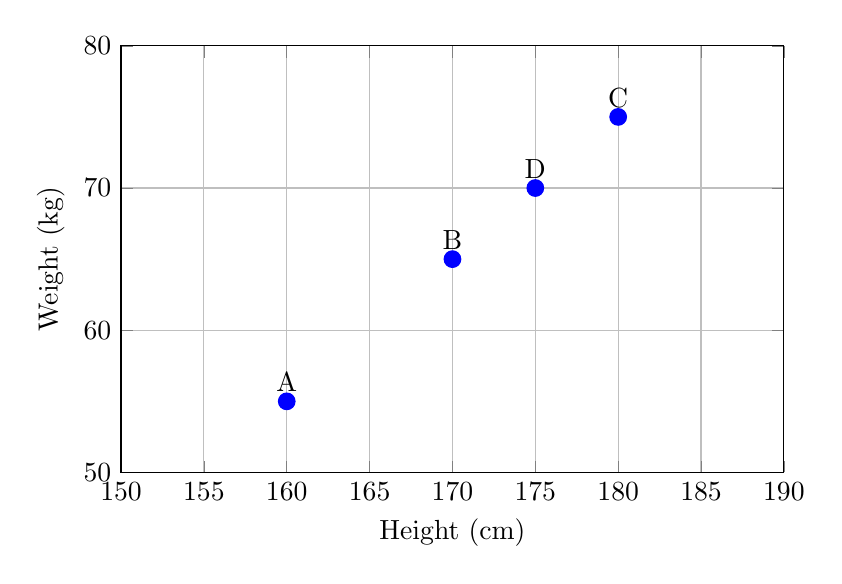
\begin{tikzpicture}
\begin{axis}[
    xlabel={Height (cm)},
    ylabel={Weight (kg)},
    xmin=150, xmax=190,
    ymin=50, ymax=80,
    grid=major,
    width=10cm,
    height=7cm
]
\addplot[only marks, mark=*, mark size=3pt, color=blue] coordinates {
    (160,55) (170,65) (180,75) (175,70)
};
\node[above] at (160,55) {A};
\node[above] at (170,65) {B};
\node[above] at (180,75) {C};
\node[above] at (175,70) {D};
\end{axis}
\end{tikzpicture}
\end{center}
\end{frame}

\begin{frame}{Linear Regression: Finding the Best Line}
\textbf{Goal:} Predict weight from height

\vspace{1em}
\textbf{Model:} $\text{weight} = \beta_0 + \beta_1 \times \text{height}$

\vspace{1em}
\textbf{Matrix form:}
\begin{align}
\underbrace{\begin{bmatrix} 55 \\ 65 \\ 75 \\ 70 \end{bmatrix}}_{\vec{y}} = 
\underbrace{\begin{bmatrix} 1 & 160 \\ 1 & 170 \\ 1 & 180 \\ 1 & 175 \end{bmatrix}}_{X} 
\underbrace{\begin{bmatrix} \beta_0 \\ \beta_1 \end{bmatrix}}_{\vec{\beta}}
\end{align}

\textbf{Matrix X converts} parameter space $(\beta_0, \beta_1)$ to prediction space!
\end{frame}

\begin{frame}{Solving Linear Regression - Step 1}
\textbf{Solution:} $\vec{\beta} = (X^T X)^{-1} X^T \vec{y}$

\vspace{1em}
\textbf{First, compute } $X^T X$:
\begin{align}
X^T X &= \begin{bmatrix} 1 & 1 & 1 & 1 \\ 160 & 170 & 180 & 175 \end{bmatrix} \begin{bmatrix} 1 & 160 \\ 1 & 170 \\ 1 & 180 \\ 1 & 175 \end{bmatrix} \\
&= \begin{bmatrix} 4 & 685 \\ 685 & 117325 \end{bmatrix}
\end{align}
\end{frame}

\begin{frame}{Solving Linear Regression - Step 2}
\textbf{Next, compute } $X^T \vec{y}$:
\begin{align}
X^T \vec{y} &= \begin{bmatrix} 1 & 1 & 1 & 1 \\ 160 & 170 & 180 & 175 \end{bmatrix} \begin{bmatrix} 55 \\ 65 \\ 75 \\ 70 \end{bmatrix} \\
&= \begin{bmatrix} 265 \\ 45425 \end{bmatrix}
\end{align}
\end{frame}

\begin{frame}{Solving Linear Regression - Step 3}
\textbf{Finally, compute } $(X^T X)^{-1} X^T \vec{y}$:

\vspace{1em}
Using the matrix inverse formula or calculator:
\begin{align}
(X^T X)^{-1} = \begin{bmatrix} 0.115 & -0.000067 \\ -0.000067 & 0.000000039 \end{bmatrix}
\end{align}

\vspace{1em}
Therefore:
\begin{align}
\vec{\beta} = (X^T X)^{-1} X^T \vec{y} = \begin{bmatrix} -105 \\ 1 \end{bmatrix}
\end{align}
\end{frame}

\begin{frame}{Linear Regression Result}
After computing $(X^T X)^{-1} X^T \vec{y}$:

\begin{align}
\vec{\beta} = \begin{bmatrix} -105 \\ 1 \end{bmatrix}
\end{align}

\vspace{1em}
\textbf{Our model:} $\text{weight} = -105 + 1 \times \text{height}$

\vspace{0.5em}
\textbf{Perfect fit:} For height 170cm: $-105 + 1(170) = 65$ kg

\vspace{1em}
\textbf{Key insight:} Matrix $X$ converts 2 parameters $(\beta_0, \beta_1)$ into 4 predictions (one for each student)!
\end{frame}

\begin{frame}{Regression Line Visualization}
\begin{center}
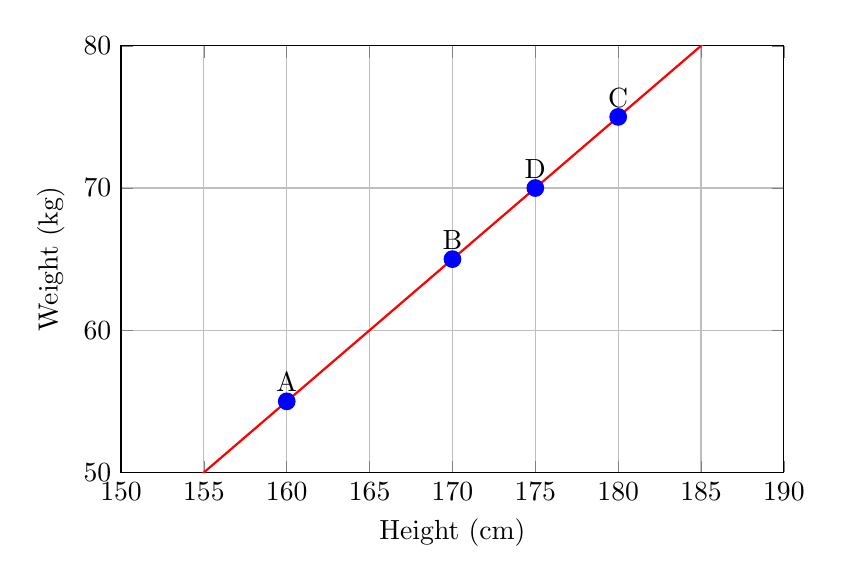
\begin{tikzpicture}
\begin{axis}[
    xlabel={Height (cm)},
    ylabel={Weight (kg)},
    xmin=150, xmax=190,
    ymin=50, ymax=80,
    grid=major,
    width=10cm,
    height=7cm
]
\addplot[only marks, mark=*, mark size=3pt, color=blue] coordinates {
    (160,55) (170,65) (180,75) (175,70)
};
\addplot[domain=150:190, samples=100, color=red, thick] {-105 + x};
\node[above] at (160,55) {A};
\node[above] at (170,65) {B};
\node[above] at (180,75) {C};
\node[above] at (175,70) {D};
\end{axis}
\end{tikzpicture}
\end{center}

The red line is our ``best fit'' through the data.
\end{frame}

\begin{frame}{From Linear Regression to PCA}
\textbf{Linear Regression asks:} What's the best line to predict $y$ from $x$?

\vspace{1em}
\textbf{PCA asks:} What's the best coordinate system for our data?

\vspace{2em}
\textbf{Key insight:}
\begin{itemize}
    \item Linear regression finds one special direction (the regression line)
    \item PCA finds \emph{all} the special directions
    \item Both use the idea of ``best fit''
\end{itemize}
\end{frame}

\begin{frame}{PCA: Best Coordinate System}
\textbf{Step 1:} Center the data (subtract the mean)

\begin{align}
\text{Mean: } \bar{\vec{v}} = \frac{1}{4}\begin{bmatrix} 685 \\ 265 \end{bmatrix} = \begin{bmatrix} 171.25 \\ 66.25 \end{bmatrix}
\end{align}

\textbf{Centered data:}
\begin{align}
\vec{v_A'} &= \begin{bmatrix} 160-171.25 \\ 55-66.25 \end{bmatrix} = \begin{bmatrix} -11.25 \\ -11.25 \end{bmatrix} \\
\vec{v_B'} &= \begin{bmatrix} -1.25 \\ -1.25 \end{bmatrix}, \quad 
\vec{v_C'} = \begin{bmatrix} 8.75 \\ 8.75 \end{bmatrix}, \quad 
\vec{v_D'} = \begin{bmatrix} 3.75 \\ 3.75 \end{bmatrix}
\end{align}
\end{frame}

\begin{frame}{Centered Data Visualization}
\begin{center}
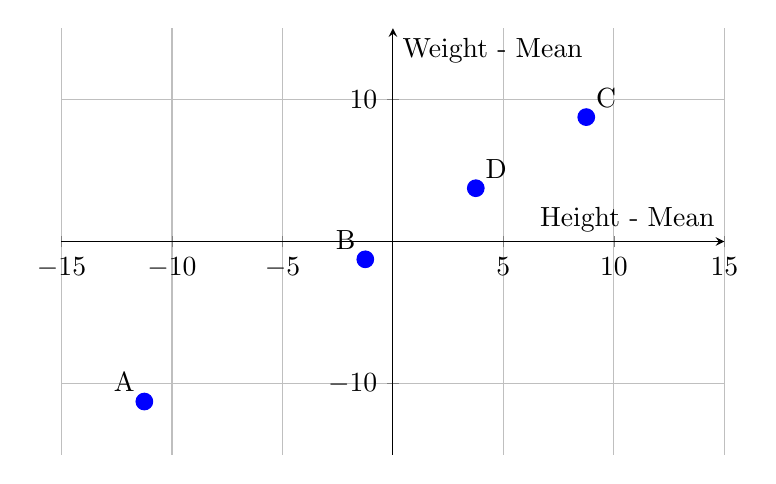
\begin{tikzpicture}
\begin{axis}[
    xlabel={Height - Mean},
    ylabel={Weight - Mean},
    xmin=-15, xmax=15,
    ymin=-15, ymax=15,
    grid=major,
    width=10cm,
    height=7cm,
    axis lines=middle
]
\addplot[only marks, mark=*, mark size=3pt, color=blue] coordinates {
    (-11.25,-11.25) (-1.25,-1.25) (8.75,8.75) (3.75,3.75)
};
\node[above left] at (-11.25,-11.25) {A};
\node[above left] at (-1.25,-1.25) {B};
\node[above right] at (8.75,8.75) {C};
\node[above right] at (3.75,3.75) {D};
\end{axis}
\end{tikzpicture}
\end{center}

Notice: all points lie roughly along a diagonal line!
\end{frame}

\begin{frame}{Finding Principal Component 1}
\textbf{Goal:} Find the direction that captures the most variation

\vspace{1em}
\textbf{Looking at our centered data:} If we draw different lines through the origin, which direction would minimize the distances from points to the line?

\vspace{1em}
\textbf{Try different angles:}
\begin{itemize}
    \item Horizontal line: points are spread out vertically
    \item Vertical line: points are spread out horizontally  
    \item Diagonal line (slope = 1): points are very close to the line!
\end{itemize}

\vspace{1em}
\textbf{The winning direction:} Along the diagonal
\begin{align}
\vec{u_1} = \frac{1}{\sqrt{2}}\begin{bmatrix} 1 \\ 1 \end{bmatrix} = \begin{bmatrix} 0.707 \\ 0.707 \end{bmatrix}
\end{align}
\end{frame}

\begin{frame}{Finding Principal Component 2}
\textbf{PC2 must be perpendicular to PC1}

\vspace{1em}
Since $\vec{u_1} = \frac{1}{\sqrt{2}}\begin{bmatrix} 1 \\ 1 \end{bmatrix}$, we have:

\begin{align}
\vec{u_2} = \frac{1}{\sqrt{2}}\begin{bmatrix} 1 \\ -1 \end{bmatrix} = \begin{bmatrix} 0.707 \\ -0.707 \end{bmatrix}
\end{align}

\vspace{1em}
\textbf{Our transformation matrix:}
\begin{align}
U = \begin{bmatrix} 0.707 & 0.707 \\ 0.707 & -0.707 \end{bmatrix}
\end{align}

This matrix converts from (height, weight) coordinates to (PC1, PC2) coordinates!
\end{frame}

\begin{frame}{PCA Transformation}
\begin{center}
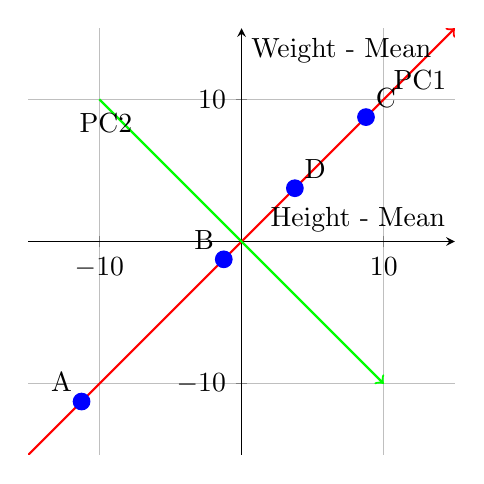
\begin{tikzpicture}
\begin{axis}[
    xlabel={Height - Mean},
    ylabel={Weight - Mean},
    xmin=-15, xmax=15,
    ymin=-15, ymax=15,
    grid=major,
    width=7cm,
    height=7cm,
    axis lines=middle
]
\addplot[only marks, mark=*, mark size=3pt, color=blue] coordinates {
    (-11.25,-11.25) (-1.25,-1.25) (8.75,8.75) (3.75,3.75)
};

% PC1 direction
\addplot[domain=-15:15, samples=2, color=red, thick, ->] {x};
\node[above right] at (10,10) {PC1};

% PC2 direction  
\addplot[domain=-10:10, samples=2, color=green, thick, ->] {-x};
\node[above left] at (-7,7) {PC2};

\node[above left] at (-11.25,-11.25) {A};
\node[above left] at (-1.25,-1.25) {B};
\node[above right] at (8.75,8.75) {C};
\node[above right] at (3.75,3.75) {D};
\end{axis}
\end{tikzpicture}
\end{center}
\end{frame}

\begin{frame}{Transform to PC Coordinates}
\textbf{Transform each point:} $\vec{v_{PC}} = U^T \vec{v'}$

\vspace{1em}
\begin{align}
U^T = \begin{bmatrix} 0.707 & 0.707 \\ 0.707 & -0.707 \end{bmatrix}
\end{align}

\textbf{Point A:}
\begin{align}
\vec{v_{A,PC}} &= \begin{bmatrix} 0.707 & 0.707 \\ 0.707 & -0.707 \end{bmatrix} \begin{bmatrix} -11.25 \\ -11.25 \end{bmatrix} \\
&= \begin{bmatrix} -15.91 \\ 0 \end{bmatrix}
\end{align}

\textbf{All points in PC coordinates:}
A: $(-15.91, 0)$, B: $(-1.77, 0)$, C: $(12.37, 0)$, D: $(5.30, 0)$
\end{frame}

\begin{frame}{The Magic of PCA}
\textbf{In original coordinates:} 4 points in 2D space

\textbf{In PC coordinates:} 4 points on a 1D line!

\vspace{1em}
\begin{center}
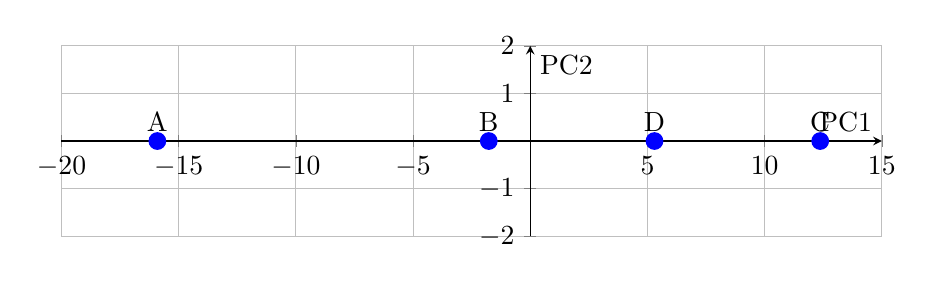
\begin{tikzpicture}
\begin{axis}[
    xlabel={PC1},
    ylabel={PC2},
    xmin=-20, xmax=15,
    ymin=-2, ymax=2,
    grid=major,
    width=12cm,
    height=4cm,
    axis lines=middle
]
\addplot[only marks, mark=*, mark size=3pt, color=blue] coordinates {
    (-15.91,0) (-1.77,0) (12.37,0) (5.30,0)
};
\node[above] at (-15.91,0) {A};
\node[above] at (-1.77,0) {B};
\node[above] at (12.37,0) {C};
\node[above] at (5.30,0) {D};
\end{axis}
\end{tikzpicture}
\end{center}

\textbf{All the variation is captured in PC1!} PC2 contributes nothing.
\end{frame}

\begin{frame}{Dimension Reduction}
\textbf{Original data:} Each student needs 2 numbers (height, weight)

\textbf{After PCA:} Each student needs only 1 number (PC1 coordinate)!

\vspace{1em}
\textbf{Reduction matrix:}
\begin{align}
\text{Keep only PC1: } \begin{bmatrix} 0.707 & 0.707 \end{bmatrix}
\end{align}

\textbf{Transform new data:}
\begin{align}
\text{New student: } \begin{bmatrix} 165 \\ 60 \end{bmatrix} \rightarrow \text{PC1 only: } -5.3
\end{align}

We've converted from 2D measurements to 1D while keeping all the important information!
\end{frame}

\begin{frame}{Matrices as Dimensional Converters}
\textbf{What we've seen:}

\vspace{1em}
\begin{itemize}
    \item \textbf{Linear regression matrix $X$:} Converts 2D parameter space $(\beta_0, \beta_1)$ to 4D prediction space
    \item \textbf{PCA transformation matrix $U^T$:} Converts 2D (height, weight) to 2D (PC1, PC2) 
    \item \textbf{Dimension reduction:} Converts 2D to 1D by keeping only important directions
\end{itemize}

\vspace{1em}
\textbf{Key insight:} Matrices are tools that convert measurements from one coordinate system to another, often revealing hidden structure in the data.
\end{frame}

\begin{frame}{Summary}
\textbf{Journey completed:}
\begin{enumerate}
    \item \textbf{Vectors as measurements:} Each data point is a vector
    \item \textbf{Linear regression:} Finding the best predictive line
    \item \textbf{Matrices as converters:} Transforming between coordinate systems  
    \item \textbf{PCA:} Finding the best coordinate system for the data
    \item \textbf{Dimension reduction:} Keeping only the important directions
\end{enumerate}

\vspace{1em}
\textbf{The power:} We went from 2D data to 1D representation without losing the essential structure!
\end{frame}

\end{document}